\subsection{Etape 1/4 : Gradients selon x et y et lissage}

Comme l'implémentation récursive proposée dans l'article est moins proche de la modélisation mathématique, nous avons décidé d'implémenter l'algorithme récursif et l'algorithme direct qui utilise des convolutions. \\

Pour l'algorithme récursif (sans convolution), nous nous sommes basé sur ce qui a été expliqué à la section
\textbf{\ref{algorithme_recursif}} \\

Pour l'algorithme direct (avec convolutions), nous nous sommes basé sur ce qui a été expliqué à la section
\textbf{\ref{algorithme_direct}}

\subsection{Etape 2/4 : Norme du gradient et direction du gradient}
\subsubsection{Norme du gradient}

\[ A(m,n)=\sqrt{r(m,n)^2 + s(m,n)^2)} \]

\[ \text{avec} \left\{\begin{array}{ll}
r \; \text{gradient selon x} \\
s \; \text{gradient selon y}
\end{array}\right. \]

\subsubsection{Direction du gradient}

\[ \emph{arg} = arctan(\frac{s(m,n)}{r(m,n)}) \]

Dans le programme que nous avons écrit, on calcule l’arc tangente entre r et s avec une fonction du langage qui retourne une valeur en degré entre $ -180 $\degre et $ 180 $\degre, ce qui correspond à l'arc tangente dans les quatre quadrants du plan.

\subsection{Etape 3/4 : Suppression des non-maxima locaux}

La suppression des non-maxima locaux est une méthode appliquée sur la norme du gradient qui permet d'affiner les contours, c'est-à-dire mettre à 0 les pixels qui ne constituent pas un contour. Un pixel de la norme du gradient est considéré comme contour s'il forme un maximum local dans la direction du gradient. \\

Soit $ \text{\emph{arg}} $ la direction du gradient en degré avec $ \text{\emph{arg}} \in [-180; 180] $. On ramène toutes les valeurs entre $ 0 $\degre et $ 180 $\degre en ajoutant $ 180 $\degre aux valeurs négatives de $ \text{\emph{arg}} $. Pour la suppression de non maxima, on ramène l'intervalle $ [0; 180] $ à quatre classes : $ 1 $, $ 2 $, $ 3 $ et $ 4 $. \\
\\
On choisit les règles suivantes : \\
\begin{itemize}
\item[•] si $ \text{\emph{arg}} \in [0; 22.5[ $ ou $ \text{\emph{arg}} \in [157.5; 180] $ alors $ \text{\emph{arg}} \in $ \textcolor{red}{\textbf{Classe 1}}
\item[•] si $ \text{\emph{arg}} \in [22.5; 67.5[ $ alors $ \text{\emph{arg}} \in $ \textcolor{blue}{\textbf{Classe 2}}
\item[•] si $ \text{\emph{arg}} \in [67.5; 112.5[ $ alors $ \text{\emph{arg}} \in $ \textcolor{green}{\textbf{Classe 3}}
\item[•] si $ \text{\emph{arg}} \in [112.5; 157.5[ $ alors $ \text{\emph{arg}} \in $ \textcolor{magenta}{\textbf{Classe 4}}
\end{itemize}

% http://www.texample.net/tikz/examples/unit-circle/
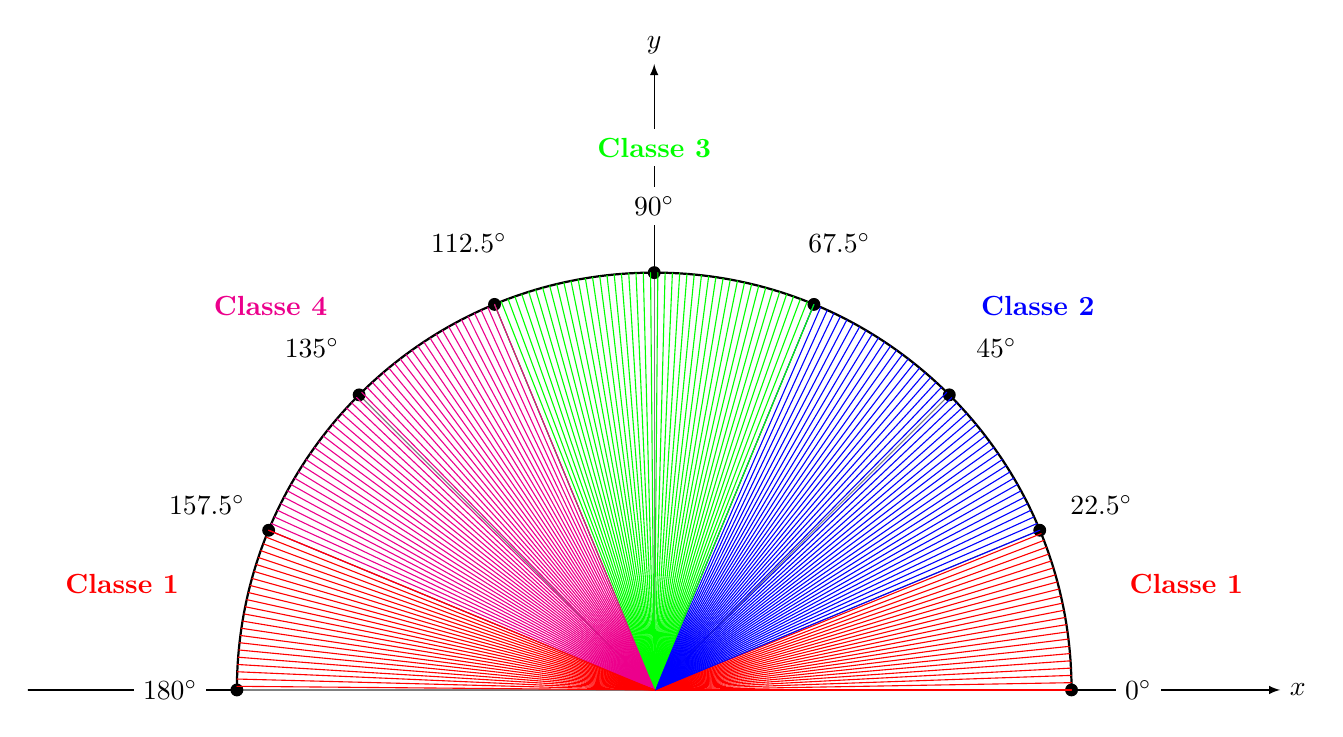
\begin{tikzpicture}[scale=5.3,cap=round,>=latex]
	% draw the coordinates
	\draw[->] (-1.5cm,0cm) -- (1.5cm,0cm) node[right,fill=white] {$x$};
	\draw[->] (0cm,0cm) -- (0cm,1.5cm) node[above,fill=white] {$y$};
	
	% draw the unit circle	
	\begin{scope}
		\clip (-1.5,0) rectangle (1.5,1.5);\clip (-1.5,0) rectangle (1.5,1.5);
		% clip permet d'avoir le demi-cercle
		\draw[thick] (0cm,0cm) circle(1cm);			
	\end{scope}
	
	\foreach \x in {0,22.5,...,180} {
		  % lines from center to point
		  \draw[gray] (0cm,0cm) -- (\x:1cm);
		  % dots at each point
		  \filldraw[black] (\x:1cm) circle(0.4pt);
		  % draw each angle in degrees
		  \draw (\x:1.16cm) node[fill=white] {$\x^\circ$};
	}
	
	\draw (11.25:1.3cm) node[fill=white] {\textcolor{red}{\textbf{Classe 1}}};	
	\draw (45:1.3cm) node[fill=white] {\textcolor{blue}{\textbf{Classe 2}}};
	\draw (90:1.3cm) node[fill=white] {\textcolor{green}{\textbf{Classe 3}}};
	\draw (135:1.3cm) node[fill=white] {\textcolor{magenta}{\textbf{Classe 4}}};
	\draw (168.75:1.3cm) node[fill=white] {\textcolor{red}{\textbf{Classe 1}}};
	
	\foreach \x in {0,1,...,22.5} {
	  % lines from center to point
	  \draw[red] (0cm,0cm) -- (\x:1cm);
	}
	
	\foreach \x in {22.5,23.5,...,67.5} {
	  % lines from center to point
	  \draw[blue] (0cm,0cm) -- (\x:1cm);
	}
	
	\foreach \x in {67.5,68.5,...,112.5} {
	  % lines from center to point
	  \draw[green] (0cm,0cm) -- (\x:1cm);
	}
	  
	\foreach \x in {112.5,113.5,...,157.5} {
	  % lines from center to point
	  \draw[magenta] (0cm,0cm) -- (\x:1cm);
	}
	
	\foreach \x in {157.5,158.5,...,180} {
	  % lines from center to point
	  \draw[red] (0cm,0cm) -- (\x:1cm);
	}
\end{tikzpicture}
\\\\
On traite ensuite les cas suivants : \\
\\
\textcolor{red}{\textbf{Classe 1}} (le contour est dans la direction Nord \--- Sud) : le pixel est un contour si la norme du gradient en ce point est supérieure au maximum de la norme du gradient des pixels Est et Ouest \\
\\
\textcolor{blue}{\textbf{Classe 2}} (le contour est dans la direction Nord-Ouest \--- Sud-Est) : le pixel est un contour si la norme du gradient en ce point est supérieure au maximum de la norme du gradient des pixels Nord-Est et Sud-Ouest \\
\\
\textcolor{green}{\textbf{Classe 3}} (le contour est dans la direction Est \--- Ouest) : le pixel est un contour si la norme du gradient en ce point est supérieure au maximum de la norme du gradient des pixels Nord et Sud \\
\\
\textcolor{magenta}{\textbf{Classe 4}} (le contour est dans la direction Nord-Est \--- Sud-Ouest) : le pixel est un contour si la norme du gradient en ce point est supérieure au maximum de la norme du gradient des pixels Nord-Ouest et Sud-Est \\
\\
Après cette étape, l'image n'est pas encore binarisée mais on a mis à 0 les pixels qui ne constituaient pas un contour.

\subsection{Etape 4/4 : Seuillage par hystérésis}

Le seuillage par hystérésis permet de retirer les faux contours. \\
\\
Pour cela, on définit deux seuils : 
\begin{itemize}
\item[•] \emph{Smin} : seuil minimum
\item[•] \emph{Smax} : seuil maximum \\
\end{itemize}

Pour chaque pixel de la norme du gradient obtenu après la suppression des non-maxima locaux, on regarde sa valeur. \\
\\
\textbf{Cas 1} : si la valeur du pixel est supérieure au seuil maximum alors ce pixel est un vrai contour donc on met sa valeur à 1 \\
\textbf{Cas 2} : si la valeur du pixel est inférieure au seuil minimum alors ce pixel est un faux contour donc on met sa valeur à 0 \\
\textbf{Cas 3} : si la valeur du pixel est entre le seuil minimum et le seuil maximum alors on regarde les valeurs des huit pixels voisins et on regarde s'il existe au moins un pixel voisin qui a une valeur supérieure au seuil maximum. Si c'est le cas, la valeur du pixel initial devient un 1 sinon 0 \\
\\
Pour le \textbf{Cas 3}, dans le code, on prend une fenêtre $3$x$3$ pour obtenir facilement les voisins du pixel au centre de cette fenêtre. \\

\begin{center}
\begin{tikzpicture}[scale=5.3,cap=round,>=latex]
        % draw the coordinates
        \draw (0.75,1.2) node[anchor=south] {\textbf{Vrai contour}};
        \draw[-] (-0.05cm,1cm) -- (1.5cm,1cm) node[right,fill=white] {\emph{Smax}};
        \draw (0.75,0.7) node[anchor=south] {\textbf{Contour incertain}};
        \draw[-] (-0.05cm,0.5cm) -- (1.5cm,0.5cm) node[right,fill=white] {\emph{Smin}};
        \draw (0.75,0.2) node[anchor=south] {\textbf{Faux contour}};
        \draw[-] (0cm,0cm) -- (1.5cm,0cm) node[right,fill=white] {};        
        \draw[->] node[below,fill=none] {$0$} (0cm,0cm) -- (0cm,1.5cm) node[above,fill=white] {$255$} ;
\end{tikzpicture}
\end{center}

L'image obtenue est maintenant binarisée. Elle contient les contours de l'image initiale et un peu de bruit.